\chapter{Relaxação Lagrangiana}
A relaxação lagrangiana procura facilitar a obtenção de LBs para um problema de otimização combinatória através da remoção de restrições dificultantes. As restrições removidas são então tratadas por meio de penalizações na função objetivo. O objetivo é obter uma versão do problema que seja mais fácil de resolver, e que sirvam como uma boa relaxação, provendo LBs que sejam o mais próximos possíveis do valor ótimo do problema original. Este capítulo apresenta uma abordagem de resolução do TSP através do método da relaxação lagrangeana. Unido ao BnB através de uma regra de \textit{branching} apropriada, o método supera o BnB combinatório do capítulo anterior em termos de performance, sendo capaz de resolver instâncias maiores.

{ 
\color{black}

\section{Relaxação de um Problema Linear Inteiro}

Considere o Problema Linear Inteiro (\textit{Integer Linear Program}, ILP) 
\begin{align*}
	\min_{x \in X} \left\{\, cx \mid Ax \geq b, Bx \geq d \,\right\}, \tag{P}\label{eq:originalProblem}
\end{align*}
em que \(X \coloneqq \left\{ \, y \in \mathbb{R}^{m} \mathbb{Z}^{n} \mid y \geq 0 \, \right\}\), i.e., a tupla $x$ representa um conjunto composto por $m$ variáveis reais e $n$ variáveis inteiras. Suponha, agora, que a presença das restrições $Ax \geq b$ impõem um desafio significativo ao problema. É possível retirar essas restrições e penalizar a função objetivo caso sejam violadas, conforme o problema
\begin{align*}
	\min_{x \in X} \left\{\, cx + \lambda (b - Ax) \mid Bx \geq d \,\right\} \tag{PR$_\lambda$}\label{eq:problemRelaxed},
\end{align*}
em que cada componente do vetor $\lambda \geq 0$ está associada a uma das restrições retiradas do problema original \eqref{eq:originalProblem}.

Embora não seja capaz de garantir que violações não ocorram, o termo adicional na função objetivo do problema \eqref{eq:problemRelaxed} incentiva que as restrições $Ax \geq b$ sejam respeitadas. Para perceber isso, seja $a_i$ a $i$-ésima linha da matriz $A$. Note que o problema em questão é de minimização, e se $a_i x < b_i$ para algum $i$, um número não negativo (i.e., uma penalização) $\lambda_i (b_i - a_i x)$ será adicionado à função objetivo, aumentando-a. 

\begin{theorem}
	\label{thm:relaxLB}
	Para qualquer $\lambda \geq 0$, \eqref{eq:problemRelaxed} é uma relaxação de \eqref{eq:originalProblem}.
\end{theorem}
\begin{proof}
	Já que \eqref{eq:originalProblem} possui todas as restrições de \eqref{eq:problemRelaxed}, então, o espaço de soluções de \eqref{eq:originalProblem} está contido no espaço de soluções de \eqref{eq:problemRelaxed}. Para mostrar que o valor ótimo de \eqref{eq:problemRelaxed} é um LB para o valor ótimo de \eqref{eq:originalProblem}, observe que, para qualquer solução viável $x$ de \eqref{eq:originalProblem}, 
	\begin{align*}
		(b - Ax) \leq 0.
	\end{align*}
	Já que foi especificado que $\lambda \geq 0$, então
	\begin{align*}
		\lambda (b - Ax) \leq 0,
	\end{align*}
	e, por consequência,
	\begin{align*}
		cx + \lambda (b - Ax) \leq cx,
	\end{align*}
	completando a demonstração.
\end{proof}

\begin{theorem}
	\label{thm:xIsOptimal}
	Se $x^*$ é uma solução ótima de \eqref{eq:problemRelaxed} para algum $\lambda \geq 0$ e $\lambda (b - Ax^*) = 0$ e $Ax^* \geq b$, então $x^*$ também é uma solução ótima de \eqref{eq:originalProblem}.
\end{theorem}
\begin{proof}
	Primeiramente, $x^*$ é viável para \eqref{eq:originalProblem}, já que $Ax^* \geq b$. Além disso, o fato de que $x^*$ é uma solução ótima para \eqref{eq:problemRelaxed} significa que
	\begin{align*}
		cx^* + \lambda (b - Ax^*) \leq cx + \lambda (b - Ax)
	\end{align*}
	para qualquer $x$, mas $\lambda (b - Ax^*) = 0$, então
	\begin{align*}
		cx^* \leq cx + \lambda (b - Ax),
	\end{align*}
	e de acordo com o Teorema \ref{thm:relaxLB}, 
	\begin{align*}
		cx + \lambda (b - Ax) \leq cx,
	\end{align*}
	logo,
	\begin{align*}
		cx^* \leq cx + \lambda (b - Ax) \leq cx,
	\end{align*}
	e $x^*$ é de fato uma solução ótima para \eqref{eq:originalProblem}.
\end{proof}

\subsection{Exemplo com ILP simples}

Considere o ILP 
\begin{align*}
	\min \left\{ 5x_1 + 4x_2 + 2x_3 \mid 2x_1 + 3x_2 + 4x_3 \geq 5, (x_1,x_2,x_3) \in \{0,1\}^3 \right\}. \tag{P1}\label{eq:ilpExample}
\end{align*}
Relaxando-se a restrição de \eqref{eq:ilpExample}, obtém-se o novo ILP
\begin{align*}
	\min \left\{ 5x_1 + 4x_2 + 2x_3 + \lambda(5 - 2x_1 + 3x_2 + 4x_3) \mid (x_1,x_2,x_3) \in \{0,1\}^3 \right\}. \tag{PR$_\lambda$1}\label{eq:ilpExampleRelax}
\end{align*} 

Já que o problema original \eqref{eq:ilpExample} possui uma única restrição, que foi removida, sua relaxação possui um único penalizador $\lambda$ na função objetivo. A solução ótima de \eqref{eq:ilpExampleRelax} depende do valor do penalizador $\lambda$, que deve ser escolhido antes da resolução do problema. Se $\lambda = 0$, por exemplo, o valor ótimo é obtido fazendo-se $x_1 = x_2 = x_3 = 0$, tornando nulo o valor da função objetivo.

Para analisar o comportamento do problema em função de $\lambda$, convém reagrupar os termos da função objetivo de \eqref{eq:ilpExampleRelax}, obtendo-se a expressão equivalente
\begin{equation}
	(5 - 2\lambda) x_1 + (4 - 3\lambda) x_2 + (2 - 4\lambda) x_3 + 5\lambda. \label{eq:ilpExampleFO}
\end{equation}
Observando-se a Expressão \eqref{eq:ilpExampleFO}, e sabendo-se que \eqref{eq:ilpExampleRelax} não possui restrições além do domínio das variáveis $x_1$, $x_2$ e $x_3$, é fácil perceber que 
\begin{align*}
	x_1 = \begin{cases}
		1 &\text{ se } \lambda > 5/2 \\
		0 &\text{ caso contrário.}
	\end{cases}
\end{align*}
Em outras palavras, fazer $x_1 = 1$ só irá diminuir a função objetivo se $5 - 2\lambda$ (termo que multiplica $x_1$ na Expressão \eqref{eq:ilpExampleFO}) for menor que zero.

Seguindo-se uma lógica similar, 
\begin{align*}
	x_2 = \begin{cases}
		1 &\text{ se } \lambda > 4/3 \\
		0 &\text{ caso contrário,}
	\end{cases}
\end{align*}
e
\begin{align*}
	x_3 = \begin{cases}
		1 &\text{ se } \lambda > 1/2 \\
		0 &\text{ caso contrário.}
	\end{cases}
\end{align*}
Dessa forma, com o intuito de determinar o valor ótimo de \eqref{eq:ilpExampleRelax}, é possível saber, para cada valor de $\lambda$, quais variáveis assumem o valor 1, e quais assumem o valor 0. A Figura \ref{fig:piecewiseKnapsack} ilustra o comportamento do valor ótimo de \eqref{eq:ilpExampleRelax} em função do penalizador $\lambda$. Observe que $\lambda = 4/3$ foi o penalizador que proveu a melhor estimativa do valor ótimo do problema original \eqref{eq:ilpExample}.

\begin{figure}[htpb!]
	\centering
	\begin{tikzpicture}[x=2cm, y=0.7cm]
		\draw[-{Triangle}, ultra thick] (0,0) -- node[pos=1.05]{$\lambda$} (3,0);
		\draw[-{Triangle}, ultra thick] (0,0) -- node[pos=1.05]{FO}(0,7);

		\node[circle, fill=black, draw=black, inner sep = 1.5pt](l1) at (0.5, 2.5) {};
		\node[circle, fill=black, draw=black, inner sep = 1.5pt](l2) at (1.3333,3.3333) {};
		\node[circle, fill=black, draw=black, inner sep = 1.5pt](l3) at (2.5,1) {};

		\node[](pot) at (2, 7){Valor ótimo de \eqref{eq:ilpExample}};
		\draw[-{Triangle}, very thick] (pot) to[out=180,in=90] (0.65,6.2);

		\draw[dashed, very thick] (0,6) -- (2.75,6);
		\draw[-, very thick] (0,0) -- (0.5, 2.5);
		\draw[-, very thick] (0.5,2.5) -- (1.33333,3.33333);
		\draw[-, very thick] (1.33333,3.33333) -- (2.5,1);
		\draw[-, very thick] (2.5,1) -- (2.75,0);

		\node[](v1) at (-0.25,0 |- l1) {5/2};
		\node[](v2) at (-0.25,0 |- l2) {10/3};
		\node[](v3) at (-0.25,0 |- l3) {1};
		\node[](v4) at (-0.25,0 |- 0,6) {6};

		\draw[dashed] (v1) -- (l1);
		\draw[dashed] (v2) -- (l2);
		\draw[dashed] (v3) -- (l3);

		\draw[-, ultra thick,draw=black] (0,-0.125 -| l1) -- (0,0.125 -| l1);
		\draw[-, ultra thick,draw=black] (0,-0.125 -| l2) -- (0,0.125 -| l2);
		\draw[-, ultra thick,draw=black] (0,-0.125 -| l3) -- (0,0.125 -| l3);

		\node[] at (0,-0.625 -| l1) {1/2};
		\node[] at (0,-0.625 -| l2) {4/3};
		\node[] at (0,-0.625 -| l3) {5/2};

	\end{tikzpicture}
	\caption{Valor da função objetivo de \eqref{eq:ilpExampleRelax} em função de $\lambda$.}
	\label{fig:piecewiseKnapsack}
\end{figure}

A próxima seção formaliza a tarefa que consiste em encontrar os melhores penalizadores para problemas como \eqref{eq:ilpExampleRelax}.

\section{Dual lagrangiano}

Um tema introduzido no capítulo anterior --- e recorrente no restante deste livro --- é a redução do \textit{gap} entre o LB provido pela relaxação e o valor ótimo do problema original. No exemplo anterior, uma análise feita a partir de um ILP revelou que o valor ótimo de sua relaxação depende diretamente do valor escolhido para o penalizador. Essa noção pode ser facilmente generalizada, e conclui-se que, ironicamente, encontrar os melhores penalizadores para \eqref{eq:problemRelaxed} pode ser formulado como o outro problema de otimização
\begin{align*}
	\max_{\lambda \geq 0} \left\{ \min_{x \in X} \left\{\, cx + \lambda (b - Ax) \mid Bx \geq d \,\right\} \right\}. \tag{D}\label{eq:dualLagrangiano}
\end{align*}

Por apresentar dois problemas de otimização interdependentes, o problema \eqref{eq:dualLagrangiano} pode parecer inicialmente confuso. Lembre-se, no entanto, de que como mostrado no exemplo anterior, o valor ótimo do problema interno depende do vetor de penalizadores $\lambda$. Em outras palavras, sendo $v\eqref{eq:problemRelaxed}$ o valor objetivo da solução ótima de \eqref{eq:problemRelaxed}, o problema \eqref{eq:dualLagrangiano} pode ser formulado alternativamente como \begin{align*}
	\max_{\lambda \geq 0} \left\{ v\eqref{eq:problemRelaxed} \right\}. \tag{D}
\end{align*}

Diferente de \eqref{eq:originalProblem} e \eqref{eq:problemRelaxed}, \eqref{eq:dualLagrangiano} possui como variáveis o vetor de penalizadores $\lambda$. Resolver \eqref{eq:dualLagrangiano} significa encontrar o melhor LB possível para o problema original \eqref{eq:originalProblem} a partir de sua relaxação \eqref{eq:problemRelaxed}. No exemplo anterior, a solução ótima para o dual lagrangiano associado a \eqref{eq:ilpExampleRelax} é $\lambda=4/3$, e o valor objetivo referente à solução é $10/3$.

Resta, então, descobrir uma maneira de resolver o dual lagrangiano. Infelizmente, embora contínua, a função na Figura \ref{fig:piecewiseKnapsack} claramente não é diferenciável, não permitindo o uso de técnicas do cálculo diferencial para determinar seus pontos máximos. No entanto, a função possui uma característica interessante: ela é côncava (i.e., a região abaixo da função forma um conjunto convexo) e, portanto, possui um ótimo global, ou seja, um único pico. Essas características, que são generalizadas para qualquer problema semelhante a $\eqref{eq:problemRelaxed}$ no seguinte teorema, serão exploradas mais adiante.

\begin{theorem}
	\label{thm:lagrangianDualConcavity}
	A função $v\eqref{eq:problemRelaxed}$ é sempre côncava.
\end{theorem}
\begin{proof}
	Qualquer ILP pode ser reformulado em função da envoltória convexa de sua região viável. Por isso, o problema \eqref{eq:problemRelaxed} pode ser reescrito como  \[ \min_{x \geq 0} \left\{ cx + \lambda (b - Ax) \mid x \in \text{Co} \left\{ x \in X \mid Bx \geq d  \right\} \right\}, \] em que $\text{Co}\{ . \}$ denota a envoltória convexa do conjunto $\{.\}$. Sabe-se, ainda, que a solução ótima de um problema linear reside em um de seus pontos extremos. Assim, sendo \(\left\{ x^1, \dots, x^K  \right\}\) o conjunto de pontos extremos de \(\text{Co} \left\{ x \in X \mid Bx \geq d \right\}\), \eqref{eq:problemRelaxed} pode ser novamente reformulado como \[ \min_{k=1,\dots,K} \left\{ cx^k + \lambda (b - Ax^k)  \right\}. \]
Isso significa que a função $v\eqref{eq:problemRelaxed}$ equivale ao mínimo de uma ou mais funções lineares de $\lambda$, sendo, portanto, côncava, de acordo com um resultado conhecido da Análise Convexa.
\end{proof}

O Teorema \ref{thm:lagrangianDualConcavity} estabelece que resolver o dual lagrangiano se reduz a encontrar o máximo global de uma função contínua. As próximas seções descrevem os passos necessários para resolver esse problema de otimização usando uma teoria análoga às técnicas vistas em cursos de Cálculo.

\section{Subgradiente}

Dada uma função côncava $f : \mathbb{R}^m \mapsto \mathbb{R} $, o vetor $g \in \mathbb{R}^m$ é considerado um subgradiente no ponto $\lambda_0 \in \mathbb{R}^m$ se
\begin{equation}
	f(\lambda) \leq g (\lambda - \lambda_0) + f(\lambda_0) \label{eq:subgradientEq}
\end{equation}
para qualquer $\lambda \in \mathbb{R}^m$. 

De acordo com a Inequação \eqref{eq:subgradientEq}, para que $g$ seja um subgradiente válido da função $f(\lambda)$ no ponto $\lambda_0$, o gráfico	da função linear
\[h(\lambda) = f(\lambda_0) + g(\lambda - \lambda_0) \] precisa estar sempre acima do gráfico de $f(\lambda)$. Isso pode ser visto mais facilmente nas figuras \ref{fig:subgrads1}--\ref{fig:subgrads2}, que apresentam exemplos de três vetores subgradientes para uma função de uma variável. Dois dos três vetores são subgradientes válidos para o ponto $\lambda = 1/2$, enquanto o outro é valido para o ponto $\lambda = 5$. Na Figura \ref{fig:subgrads1}, as retas tracejadas representam o gráfico da função $h(\lambda)$ para cada vetor subgradiente. Note que tais funções obedecem à Inequação \eqref{eq:subgradientEq}, sendo sempre maiores ou iguais à função $f(\lambda)$. Os vetores ortogonais a tais retas não são exatamente os subgradientes em si, mas extensões deles: já que $f(\lambda)$ é uma função de uma única variável, os subgradientes devem pertencer a $\mathbb{R}$. Os verdadeiros subgradientes, que são vetores unidimensionais no caso do exemplo, se encontram na Figura \ref{fig:subgrads2}, espalhados verticalmente para melhor visualização.

\begin{figure}[htpb!]
	\centering
	\subfloat[]{
		\scalebox{1}{
	\begin{tikzpicture}[x=1cm,y=1cm]
		\draw[-{Triangle}, ultra thick] (0,0) -- node[pos=1.05]{$\lambda$} (6,0);
		\draw[-{Triangle}, ultra thick] (0,0) -- node[pos=1.1]{$f(\lambda)$}(0,3.8);

		\draw[dashed, very thick, draw=blue] (0, 1) -- (1, 3+1);
		\draw[-{Triangle}, very thick, draw=blue] (1/2, 5/2) -- (1/2 + 3/1, 5/2 -1/1);
		\draw[dashed, very thick, draw=red] (0, 1.8) -- (1, 1.4 + 1.8);
		\draw[-{Triangle}, very thick, draw=red] (1/2, 5/2) --  (1/2 + 1.4/1, 5/2 -1/1);
		\draw[dashed, very thick, draw=purple] (4, 2.33333) -- (5.75, 0);
		\draw[-{Triangle}, very thick, draw=purple] (5, 1) --  (5 -4/3, 1 -1/1);

		\node[circle, fill=black, draw=black, inner sep = 1.5pt](l1) at (0.5, 2.5) {};
		\node[circle, fill=black, draw=black, inner sep = 1.5pt](l2) at (2.6666,3.3333) {};
		\node[circle, fill=black, draw=black, inner sep = 1.5pt](l3) at (5,1) {};

		\draw[-, very thick] (0,0) -- (l1);
		\draw[-, very thick] (l1) -- (l2);
		\draw[-, very thick] (l2) -- (l3);
		\draw[-, very thick] (l3) -- (5.5,0);

		\draw[-, ultra thick,draw=black] (0,-0.125 -| l1) -- (0,0.125 -| l1);
		\draw[-, ultra thick,draw=black] (0,-0.125 -| l2) -- (0,0.125 -| l2);
		\draw[-, ultra thick,draw=black] (0,-0.125 -| l3) -- (0,0.125 -| l3);

		\node[] at (0,-0.625 -| l1) {1/2};
		\node[] at (0,-0.625 -| l2) {8/3};
		\node[] at (0,-0.625 -| l3) {5};

		\node[rectangle, draw=black, rounded corners=2pt, thick, fill=white, fill opacity=1] (h2) at (2.5, -1.35) {$f(1/2) + {\color{red}\mathbf{1.4}} (\lambda-1/2)$};
		\node[rectangle, draw=black, rounded corners=2pt, thick, fill=white, fill opacity=1] (h3) at (5.2,3) {$f(5) + ({\color{purple}\mathbf{-4/3}})(\lambda - 5)$};
		\node[rectangle, draw=black, rounded corners=2pt, thick, fill=white, fill opacity=1] (h1) at (2.9, 4.5) {$f(1/2) + {\color{blue}\mathbf{3}}(\lambda-1/2)$};
		\draw[->] (h3) to [bend left] (5,1.5);
		\draw[->] (h1) to [bend left] (1,3.5);
		\draw[->] (h2.west) to [out=180,in=225] (-0.125,1.7);



	\end{tikzpicture}
}

	\label{fig:subgrads1}
} 
%\hspace{0.125cm}
	\subfloat[]{
		\scalebox{0.75}{
	\begin{tikzpicture}[x=1cm,y=1cm]
		\draw[dashed] (1/2, 1) -- (1/2, -1);
		\draw[dashed] (5, 2) -- (5, -1);

		\draw[-{Triangle}, ultra thick, color=blue] (1/2,0) -- node[pos=0.5, yshift=-0.525cm, fill=white]{$g^1 = 3$} (1/2+3,0);
		\draw[-{Triangle}, ultra thick, color=red] (1/2,1) -- node[pos=0.5, yshift=0.525cm, fill=white]{$g^2 = 1.4$} (1/2+1.4,1);
		\draw[-{Triangle}, ultra thick, color=purple] (5,2) -- node[pos=0.5, yshift=0.525cm, fill=white]{$g^3 = -4/3$} (5-4/3,2);
		\draw[-{Triangle}, ultra thick] (0, -1) -- node[pos=1.05]{$\lambda$} (6,-1);

		% \node[circle, inner sep = 0.1cm, draw=black,fill=black] (ogb) at (8/3,-1) {};
		% \node[] (og) at (8/3,-1.5) {ótimo global};
		% \draw[->, thick] (og) to[bend right] (2.8, -1.1);

		\draw[-, ultra thick,draw=black] (0, -1 -0.125 -| 1/2, -1) -- node[pos=-1.5]{$1/2$}(0, -1 + 0.125 -| 1/2, -1);
		\draw[-, ultra thick,draw=black] (0, -1 -0.125 -| 5, -1) -- node[pos=-1.5]{$5$} (0, -1 + 0.125 -| 5, -1);
		\draw[-, ultra thick,draw=black] (0, -1 -0.125 -| 8/3, -1) -- node[pos=-1.5]{$8/3$} (0, -1 + 0.125 -| 8/3, -1);

	\end{tikzpicture}
}

	\label{fig:subgrads2}
}

	\caption{Exemplos de vetores subgradientes para uma função côncava de uma variável}
	\label{fig:exemplosSubrad}
\end{figure}

A informação mais importante a ser extraída da Figura \ref{fig:subgrads2} é que, olhando-se a partir do ponto $\lambda_0$, o subgradiente associado ``aponta'' para o ótimo global de $f(\lambda)$ ($8/3$). Na verdade, se $f(\lambda)$ for uma função diferenciável de uma única variável, o subgradiente no ponto  $\lambda_0$ é exatamente $df(\lambda_0)/d\lambda$. O vetor subgradiente nada mais é, portanto, que uma generalização do conceito de gradiente para funções côncavas não diferenciáveis. Dessa forma, uma maneira de resolver o dual lagrangiano é começar a partir de um ponto $\lambda_0$ e ``dar um pequeno passo'' na direção do vetor subgradiente até o ponto $\lambda_0 + \epsilon g$, em que $\epsilon$ é um número muito pequeno. Repetindo-se o processo até que o aumento no $f(\lambda)$ seja marginal, é possível chegar ao ótimo global. 

\begin{theorem}
	\label{thm:axbSubgrad}
	Se $x^*$ é a solução ótima de \eqref{eq:problemRelaxed} para $\lambda = \lambda_0$, então $b - Ax^*$ é subgradiente de \eqref{eq:dualLagrangiano} no ponto $\lambda_0$.
\end{theorem}
\begin{proof}
Sejam $f(\lambda)$ e $f(\lambda_0)$ os valores de $v\eqref{eq:problemRelaxed}$ para os penalizadores $\lambda$ e $\lambda_0$, respectivamente. Sabe-se que,
\begin{align*}
	f(\lambda_0) &= \min_{x\in X}\{\, cx + \lambda_0(b - Ax) \mid Bx \geq d \, \}\\
	 &= cx^* + \lambda_0 (b - Ax^*).
	% z(\text{PR}_{\lambda}) \leq (Ax^* - b) (\lambda - \lambda_0) + z(\text{PR}_{\lambda_0})
\end{align*}
Além disso embora a solução $x^*$ seja ótima para \eqref{eq:problemRelaxed} quando o penalizador é $\lambda_0$, isso não necessariamente é verdade para o penalizador arbitrário $\lambda$. Portanto,
\begin{align*}
	f(\lambda) & \leq cx^* + \lambda (b - Ax^*) \\
	& \leq cx^* + \lambda(b - Ax^*) + \lambda_0(b - Ax^*) - \lambda_0(b - Ax^*) \\
	& \leq f(\lambda_0) + \lambda(b - Ax^*) - \lambda_0 (b - Ax^*) \\
	& \leq (b - Ax^*) (\lambda - \lambda_0) + f(\lambda_0), 
\end{align*}
e o vetor $g = (b - Ax^*)$ é de fato um subgradiente válido no ponto $\lambda_0$, de acordo com a definição de subgradiente.
\end{proof}

O Teorema \ref{thm:axbSubgrad} nos dá uma maneira simples e direta de obter um vetor subgradiente para qualquer ponto $\lambda$. Em posse disso, o procedimento para resolver o dual lagrangiano, que baseia-se na ideia descrita anteriormente, é apresentado na próxima seção.

\section{Método do subgradiente}

Como discutido na seção anterior, a ideia por trás do método de resolução do dual lagrangiano é caminhar em direção ao ótimo global de \eqref{eq:dualLagrangiano} através do vetor subgradiente. O procedimento depende, dentre outros fatores, de um cálculo de um tamanho de passo e de um critério de parada adequado, para que possa convergir numa velocidade razoável. Uma das maneiras de implementar esse procedimento, proposta em \referencia{}, é descrita no Algoritmo \ref{alg:subgradMethod}.

\begin{algorithm}[ht]
\DontPrintSemicolon
\KwData{..}
\KwResult{$\lambda^*$}
\Begin{
	$\text{UB} \gets \text{Heuristic upper bound for original problem}$ \label{dualSolveStart1}\;
	$\lambda \gets 0$ \;
	$\epsilon \gets 1$ \;
	$k \gets 0$ \label{dualSolveStart2} \;
	\While{stop criterion not met}{
		$x^* \gets \text{optimal solution of } \eqref{eq:problemRelaxed}$ \; \label{solveRelaxation}
		$w \gets cx^* + \lambda (b - Ax^*) \label{getRelaxationLB} $ \; 
		$\lambda \gets \lambda + \mu \left( b - Ax^* \right)$  \label{updateStepDirection}\; 
		$\mu \gets \epsilon (\text{UB} - w) / \left( (b - Ax^*) (b - Ax^*) \right)$  \label{updateStepSize}\; 

		\If{$w > w^*$}{ \label{atualizaMelhorLB1}
			$w^* \gets w$ \;
			$\lambda^* \gets \lambda$ \;
			$k \gets 0$ \label{atualizaMelhorLB2}\; 
		}
		\Else{
			$k \gets k + 1$ \label{incrementaNumIteracoes}\;
			\If{$k \geq k_{\text{max}}$}{ \label{numMaxIter1}
				$k \gets 0$ \;
				$\epsilon \gets \epsilon / 2$ \label{numMaxIter2} \;
			}
		}
		$\text{stop criterion} \gets \epsilon < \epsilon_{\text{min}} \text{ or } (Ax^* \geq b \text{ and } \lambda (b - Ax^*) = 0)$ \;
	}

	\Return{$\lambda^*$} \;
}
\caption{\textsc{Subgradient Method}\label{alg:subgradMethod}}
\end{algorithm}

No Algoritmo, \ref{alg:subgradMethod}, inicia-se com um UB obtido de maneira heurística na linha \ref{dualSolveStart1}. Após isso, a solução ótima de \eqref{eq:problemRelaxed} e seu LB asociado são obtidos nas linhas \ref{solveRelaxation}--\ref{getRelaxationLB}. Então, um pequeno passo na direção do subgradiente $b - Ax^*$ é dado na linha \ref{updateStepDirection}. O fator que determina o tamanho do passo é o número real $\mu$, que é atualizado na linha \ref{updateStepSize}. Se o LB obtido na iteração atual for melhor que o melhor LB $w^*$, então $w^*$ e  $\lambda^*$ são atualizados, e o número de iterações $k$ é resetado (linhas \ref{atualizaMelhorLB1}--\ref{atualizaMelhorLB2}). Caso contrário, o número de iterações é incrementado na linha \ref{incrementaNumIteracoes}. Além disso, se o valor do LB não melhorar (i.e., o valor objetivo do dual lagrangiano não aumentar) após  $k_{\text{max}}$ iterações, o número de iterações é resetado e o valor de $\epsilon$ é reduzido pela metade (linhas \ref{numMaxIter1}--\ref{numMaxIter2}), resultando em tamanhos de passo cada vez menores. 

O processo se repete até que o valor de $\epsilon$ seja menor que um valor muito pequeno $\epsilon_{\text{min}}$. Isso significa que o algoritmo convergiu, e a solução $\lambda$ não pode ser melhorada de forma significativa, sendo suficientemente próxima do ótimo global. Outra possibilidade (mais rara) é a de que condições semelhantes às estabelecidas no Teorema \ref{thm:xIsOptimal} sejam atingidas, %e a solução $x^*$ seja ótima para o problema original \eqref{eq:originalProblem}, 
caso no qual o Algoritmo também encerra.

\section{Qualidade do Dual Lagrangiano}

O dual lagrangiano neste capítulo foi introduzido a partir de um ILP. Sendo assim, é natural se perguntar o quão bom o LB obtido ao resolver o problema é se comparado a outras relaxações. A relaxação mais intuitiva de \eqref{eq:originalProblem} é, definitivamente, sua relaxação linear
\begin{align*}
	\min_{x \geq 0} \left\{\, cx \mid Ax \geq b, Bx \geq d \,\right\}, \tag{$\text{P}_\text{lin}$}\label{eq:linearRelax}
\end{align*}
que difere de \eqref{eq:originalProblem} apenas pelo fato de que todas as variáveis  agora pertencem ao conjunto dos números reais.
\begin{theorem}
	\label{thm:dualBetterThanLin}
	O valor ótimo de \eqref{eq:dualLagrangiano} é maior ou igual ao valor ótimo de \eqref{eq:linearRelax}. 
\end{theorem}
\begin{proof}
	O problema \eqref{eq:problemRelaxed} se torna menos restrito retirando-se suas restrições de integralidade. Portanto,
	\begin{align*}
		\max_{\lambda \geq 0} \left\{ \min_{x \in X}\left\{\, cx + \lambda(b - Ax) \mid Bx \geq d\,\right\} \right\} \geq \max_{\lambda \geq 0} \left\{ \min_{x \geq 0}\left\{\, cx + \lambda(b - Ax) \mid Bx \geq d\,\right\} \right\}.
	\end{align*}
	Observe, ainda, que o lado direito da inequação acima pode ser reescrito como
	\begin{align*}
		\max_{\lambda \geq 0} \left\{ \lambda b + \min_{x \geq 0}\left\{\, (c - \lambda A) x ) \mid Bx \geq d\,\right\} \right\}.
	\end{align*}
	Substituindo-se o problema de minimização interno pelo seu dual, o problema anterior pode ser reescrito novamente como
	\begin{align*}
		\max_{\lambda \geq 0} \left\{ \lambda b + \max_{y \geq 0}\left\{\, yd  \mid yB \leq (c - \lambda A) \,\right\} \right\} = \max_{\lambda \geq 0, y \geq 0} \left\{ \lambda b + yd  \mid yB + \lambda A\leq c \, \right\}.
	\end{align*}
	Por fim, substituindo-se o problema resultante pelo seu dual, obtém-se
	\begin{align*}
		\min_{x \geq 0} \left\{ cx  \mid Ax \geq b, Bx \geq d \, \right\},
	\end{align*}
	que é exatamente o problema \eqref{eq:linearRelax}.
\end{proof}

O Teorema \ref{thm:dualBetterThanLin} é muito importante, pois estabelece que, no pior dos casos, o LB fornecido pelo dual lagrangiano de um ILP é tão bom quanto o LB fornecido pela sua relaxação linear, podendo, por vezes, ser ainda melhor. Uma consequência direta disso é que se \eqref{eq:originalProblem} já for um problema linear (i.e., $X = \left\{ \, x \in \mathbb{R}^{m+n} \mid  x\geq 0 \,\right\}$), então o valor ótimo de \eqref{eq:dualLagrangiano} é igual ao de \eqref{eq:originalProblem}.	O seguinte Teorema permite compreender mais profundamente a qualidade do LB associado ao dual lagrangiano.

\begin{theorem}
	\label{thm:dualIsCG}
	O problema linear 
\begin{align*}
	\min_{x\geq 0} \left\{ \, cx \mid Ax \geq b, x \in \text{Co}\left\{\, Bx \geq d \mid x \in X\,\right\}\, \right\} \tag{CG}\label{eq:probCG}
\end{align*}
possui o mesmo valor ótimo que \eqref{eq:dualLagrangiano}.
\end{theorem}
\begin{proof}
	O dual lagrangiano de \eqref{eq:probCG} é
\begin{align*}
	\max_{\lambda \geq 0} \left\{\min_{x\geq 0} \left\{ \, cx + \lambda(b - Ax) \mid x \in \text{Co}\left\{\, Bx \geq d \mid x \in X\,\right\}\, \right\} \right\},
\end{align*}
e pode ser reescrito como
\begin{align*}
	\max_{\lambda \geq 0} \left\{\min_{x \in X} \left\{ \, cx + \lambda(b - Ax) \mid Bx \geq d \, \right\} \right\}, 
\end{align*}
que é exatamente igual ao problema \eqref{eq:dualLagrangiano}. Observe, ainda, que \eqref{eq:probCG} é um problema puramente linear. Portanto, segue do Teorema \ref{thm:dualBetterThanLin} que, como discutido anteriormente, a solução ótima de \eqref{eq:dualLagrangiano} possui o mesmo valor objetivo que a solução ótima de \eqref{eq:probCG}.
\end{proof}

O resultado descrito no Teorema \ref{thm:dualIsCG} estabelece uma equivalência entre \eqref{eq:dualLagrangiano} e \eqref{eq:probCG}. Essencialmente, um problema é dual do outro. Observe que  embora seja claramente uma relaxação de \eqref{eq:originalProblem},  \eqref{eq:probCG} não é meramente uma relaxação linear de \eqref{eq:originalProblem}. A diferença entre \eqref{eq:linearRelax} e \eqref{eq:probCG} é que o último captura os pontos inteiros do conjunto $\left\{\, Bx \geq d \mid x \in X \,\right\}$ por meio de uma envoltória convexa. Se, no entanto,  \[\left\{ \, Bx \geq d \mid x \geq 0 \,\right\} = \text{Co}\left\{\, Bx \geq d \mid x \in X \,\right\},\] diz-se que o problema original \eqref{eq:originalProblem} possui a Propriedade da Integralidade. Nesse caso, \eqref{eq:probCG}, \eqref{eq:dualLagrangiano} e \eqref{eq:linearRelax} todos fornecerão exatamente o mesmo LB. Para um melhor entendimento, consulte a Figura \ref{fig:figuraMonique}, que resume as informações discutidas por meio de uma interpretação geométrica.

\begin{figure}[!ht]
	\caption{Representação geométrica das relaxações de \eqref{eq:originalProblem}}
		\label{fig:figuraMonique}
\end{figure}

\section{Relaxação e dual lagrangiano do TSP}

Suponha que a variável binária $x_{ij}$ assume o valor 1 se uma aresta de um grafo completo $G = (V,E)$ for utilizada. A partir dessa variável, o TSP pode ser formulado como o ILP
\begin{align}
	\min & \sum_{i \in V, j > i} c_{ij} x_{ij}  \tag{TSP}\label{eq:probTSP} \\
	\text{s.t. } & \sum_{j>i} x_{ij} + \sum_{j<i} x_{ji} = 2, i \in V, \label{eq:degreeConstraintsTSP} \\
	& \sum_{i \in S}\sum_{j \notin S} x_{ij} \geq 1, S \subset V, S \neq \emptyset, \label{eq:subtourConstraintsTSP} \\
	& x_{ij} \in \{0,1\}, i \in V, j > i. \label{eq:integralityConstraintsTSP}
\end{align}
Na formulação \eqref{eq:probTSP}, a função objetivo visa minimizar o custo total de viagem. As restrições \eqref{eq:degreeConstraintsTSP} impõem que o grau de todos os vértices do grafo resultante seja igual a 2. As restrições \eqref{eq:subtourConstraintsTSP}, por sua vez, garantem que o grafo resultante será conexo, e portanto, formará um ciclo Hamiltoniano. Por fim, as restrições \eqref{eq:integralityConstraintsTSP} descrevem a natureza das variáveis $x_{ij}$. 

Neste caso, convém relaxar as restrições de grau para todos os vértices exceto o vértice $i = 0$. Isso significa que, na versão relaxada de \eqref{eq:probTSP} abordada neste capítulo, as restrições \eqref{eq:degreeConstraintsTSP} serão removidas para todos os vértices $i \in V, i \neq 0$. Note, porém, que as restrições \eqref{eq:probTSP} são de igualdade. É possível, porém, reescrevê-las através de duas desigualdades como
\begin{equation}
\begin{aligned}
	\sum_{j>i} x_{ij} + \sum_{j<i} x_{ji} &\geq 2, i \in V,  \\
	-\sum_{j>i} x_{ij} - \sum_{j<i} x_{ji} &\geq -2, i \in V. 
\end{aligned}\tag{\ref{eq:degreeConstraintsTSP}}
\end{equation}

A relaxação lagrangiana de \eqref{eq:probTSP} pode então ser escrita como
\begin{align}
	\min & \sum_{i \in V, j > i} c_{ij} x_{ij} + \sum_{i > 0} \lambda^1_i \left(2 - \sum_{j>i} x_{ij} - \sum_{j<i} x_{ji}\right)  \nonumber \\
			 &+ \sum_{i>0} \lambda^2_i \left(-2 + \sum_{j>i} x_{ij} + \sum_{j<i} x_{ji}\right) \tag{TSP$_\lambda$}\label{eq:probRelaxTSP} \\
	\text{s.t. } & \sum_{j>0} x_{0j} = 2, \label{} \\
	& \sum_{i \in S}\sum_{j \notin S} x_{ij} \geq 1, S \subset V, S \neq \emptyset, \label{} \\
	& x_{ij} \in \{0,1\}, i \in V, j > i. \label{}
\end{align}
A formulação \eqref{eq:probRelaxTSP} possui dois vetores de penalização $\lambda_1$ e $\lambda_2$, associados às versões com desigualdade das restrições \eqref{eq:degreeConstraintsTSP}. É possível simplificar a função objetivo significativamente reorganizando-se os termos e obtendo-se a expressão equivalente
\begin{align*}
	\sum_{i \in V, j > i} c_{ij} x_{ij} + \sum_{i > 0} \lambda^1_i \left(2 - \sum_{j>i} x_{ij} - \sum_{j<i} x_{ji}\right)	- \sum_{i>0} \lambda^2_i \left(2 - \sum_{j>i} x_{ij} - \sum_{j<i} x_{ji}\right),
\end{align*}
ou, ainda,
\begin{align*}
	\sum_{i \in V, j > i} c_{ij} x_{ij} + \sum_{i > 0} (\lambda^1_i - \lambda^2_i) \left(2 - \sum_{j>i} x_{ij} - \sum_{j<i} x_{ji}\right).
\end{align*}
Note que se $\lambda_i^1 \geq 0$ e $\lambda_i^2 \geq 0$, então $\lambda_i^1 - \lambda_i^2$ pode assumir qualquer valor real. Portanto, é possível substituir o termo $(\lambda_i^1 - \lambda_i^2)$ por um único vetor $\lambda$ cujas componentes são irrestritas (e não apenas maiores ou iguais a zero) e obter a expressão
\begin{align*}
	\sum_{i \in V, j > i} c_{ij} x_{ij} + \sum_{i > 0} \lambda_i \left(2 - \sum_{j>i} x_{ij} - \sum_{j<i} x_{ji}\right),
\end{align*}
o que faz sentido, já que diferente das restrições do tipo $Ax \geq b$, que podem ser violadas somente se $Ax < b$, as restrições de igualdade como \eqref{eq:degreeConstraintsTSP} podem ser violadas tanto para ``mais'' quanto para ``menos'', e é necessário penalizá-las conforme adequado. Reorganizando-se novamente, e supondo a existência de um penalizador ``\textit{dummy}'' $\lambda_0 = 0$, obtém-se a expressão 
\begin{align}
	\sum_{i \in V, j > i} c_{ij} x_{ij} - \sum_{i \in V} \lambda_i \left( \sum_{j>i} x_{ij} + \sum_{j<i} x_{ji} \right) + 2 \sum_{i>0} \lambda_i \label{eq:exprObjTSPLagrang1},
\end{align}

Analisando-se a Expressão \eqref{eq:exprObjTSPLagrang1}, pode-se perceber que cada termo $x_{ij}$ é multiplicado não só pelo respectivo fator $c_{ij}$, mas também pelos fatores $-\lambda_i$ e $-\lambda_j$. Finalmente, o problema \eqref{eq:probRelaxTSP} pode ser formulado como
\begin{align}
	\min & \sum_{i \in V, j > i} (c_{ij} - \lambda_i - \lambda_j) x_{ij} + 2 \sum_{i > 0} \lambda_i \tag{TSP$_\lambda$} \\
	\text{s.t. } & \sum_{j>0} x_{0j} = 2, \label{} \\
	& \sum_{i \in S}\sum_{j \notin S} x_{ij} \geq 1, S \subset V, S \neq \emptyset, \label{} \\
	& x_{ij} \in \{0,1\}, i \in V, j > i. \label{}
\end{align}
Em suma, \eqref{eq:probRelaxTSP} se resume a encontrar um grafo conexo no conjunto de vértices  $V' = \{1,2,\dots,n\}$ e conectá-lo ao nó $i=0$ por meio de exatamente duas arestas. O custo de cada aresta $\{i,j\}$ depende de $c_{ij}$ e dos  penalizadores $\lambda_i$ e $\lambda_j$, e a soma total dos custos do grafo obtido deve ser mínima. 

Exemplos de soluções para uma instância do \eqref{eq:probRelaxTSP} podem ser vistas nas Figuras \ref{fig:tsp1tree1}--\ref{fig:tsp1tree3}. Como esperado, em todos os exemplos, o nó $i=0$ está sempre conectado a exatamente outros dois nós. As figuras diferem, principalmente, no número de nós que viola as restrições  \eqref{eq:degreeConstraintsTSP}. Na Figura \ref{fig:tsp1tree1}, por exemplo, os nós 8, 3 e 7 possuem grau 3, enquanto os nós 5, 4 e 6 possuem grau 1. A Figura \ref{fig:tsp1tree2}, por outro lado, possui menos violações, com a maioria dos nós tendo grau 2, com exceção dos nós 8, 4, 7 e 2. Por fim, a Figura \ref{fig:tsp1tree3} mostra uma solução viável tanto para \eqref{eq:probRelaxTSP} quanto para \eqref{eq:probTSP}, não violando nenhuma restrição de grau.


% \begin{align*}
% 	\min \left\{\, \sum_{j > i} c_{ij} x_{ij} \big| \sum_{j>i} x_{ij} + \sum_{j<i} x_{ji} = 2, i \in V, \sum_{} \,\right\}
% \end{align*}

\begin{figure}[!ht]
	\centering
	\subfloat[]{
		\scalebox{0.7}{
		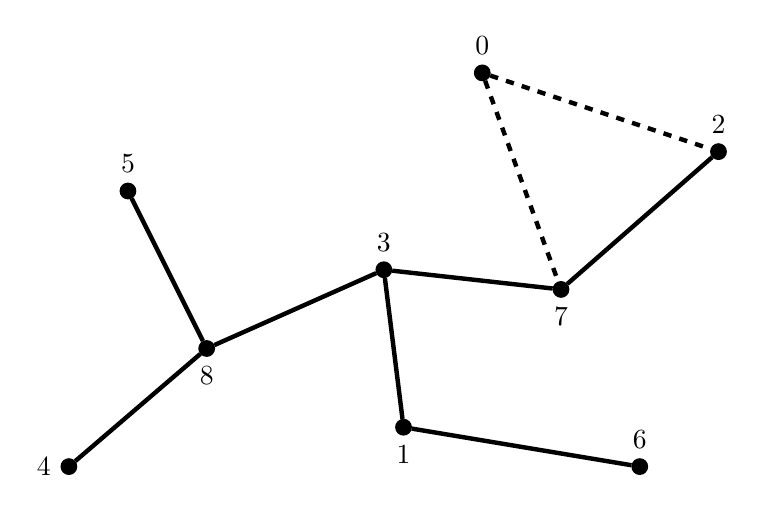
\begin{tikzpicture}
			\node[circle, draw=black, fill=black, inner sep = 2pt, label={above:0}](v0) at (2,3) {};
			\node[circle, draw=black, fill=black, inner sep = 2pt, label={below:1}](v1) at (1,-1.5) {};
			\node[circle, draw=black, fill=black, inner sep = 2pt, label={above:2}](v2) at (5,2) {};
			\node[circle, draw=black, fill=black, inner sep = 2pt, label={above:3}](v3) at (0.75,0.5) {};
			\node[circle, draw=black, fill=black, inner sep = 2pt, label={left:4}](v4) at (-3.25,-2) {};
			\node[circle, draw=black, fill=black, inner sep = 2pt, label={above:5}](v5) at (-2.5,1.5) {};
			\node[circle, draw=black, fill=black, inner sep = 2pt, label={above:6}](v6) at (4,-2) {};
			\node[circle, draw=black, fill=black, inner sep = 2pt, label={below:7}](v7) at (3,0.25) {};
			\node[circle, draw=black, fill=black, inner sep = 2pt, label={below:8}](v8) at (-1.5,-0.5) {};

			\draw[-, ultra thick] (v3) -- (v1);
			\draw[-, ultra thick] (v3) -- (v8);
			\draw[-, ultra thick] (v8) -- (v5);
			\draw[-, ultra thick] (v4) -- (v8);
			\draw[-, ultra thick] (v1) -- (v6);
			\draw[-, ultra thick] (v3) -- (v7);
			\draw[-, ultra thick] (v2) -- (v7);
			\draw[dashed, ultra thick] (v0) -- (v2);
			\draw[dashed, ultra thick] (v0) -- (v7);
		\end{tikzpicture}
	}
		\label{fig:tsp1tree1}
	}\hfill
	\subfloat[]{
		\scalebox{0.7}{
		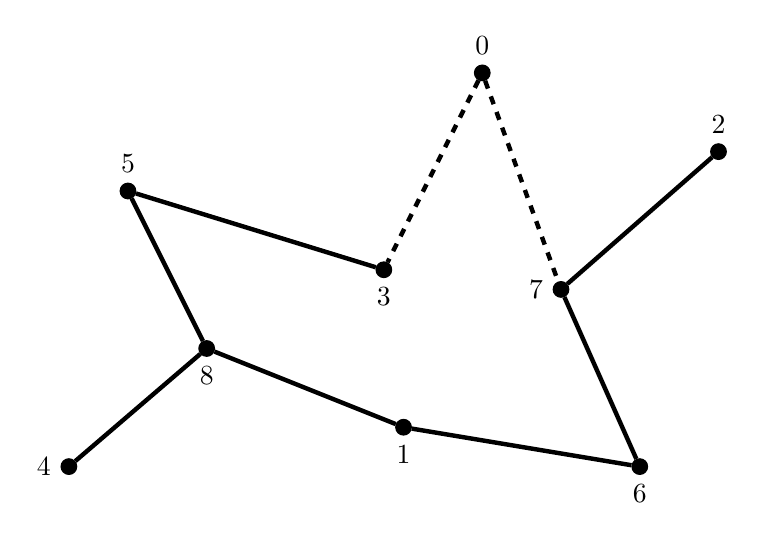
\begin{tikzpicture}
			\node[circle, draw=black, fill=black, inner sep = 2pt, label={above:0}](v0) at (2,3) {};
			\node[circle, draw=black, fill=black, inner sep = 2pt, label={below:1}](v1) at (1,-1.5) {};
			\node[circle, draw=black, fill=black, inner sep = 2pt, label={above:2}](v2) at (5,2) {};
			\node[circle, draw=black, fill=black, inner sep = 2pt, label={below:3}](v3) at (0.75,0.5) {};
			\node[circle, draw=black, fill=black, inner sep = 2pt, label={left:4}](v4) at (-3.25,-2) {};
			\node[circle, draw=black, fill=black, inner sep = 2pt, label={above:5}](v5) at (-2.5,1.5) {};
			\node[circle, draw=black, fill=black, inner sep = 2pt, label={below:6}](v6) at (4,-2) {};
			\node[circle, draw=black, fill=black, inner sep = 2pt, label={left:7}](v7) at (3,0.25) {};
			\node[circle, draw=black, fill=black, inner sep = 2pt, label={below:8}](v8) at (-1.5,-0.5) {};

			\draw[-, ultra thick] (v8) -- (v5);
			\draw[-, ultra thick] (v8) -- (v4);
			\draw[-, ultra thick] (v8) -- (v1);
			\draw[-, ultra thick] (v5) -- (v3);
			\draw[-, ultra thick] (v1) -- (v6);
			\draw[-, ultra thick] (v7) -- (v6);
			\draw[-, ultra thick] (v7) -- (v2);
			\draw[dashed, ultra thick] (v0) -- (v3);
			\draw[dashed, ultra thick] (v0) -- (v7);
		\end{tikzpicture}
	}
		\label{fig:tsp1tree2}
	}\hfill
	\subfloat[]{
		\scalebox{0.7}{
		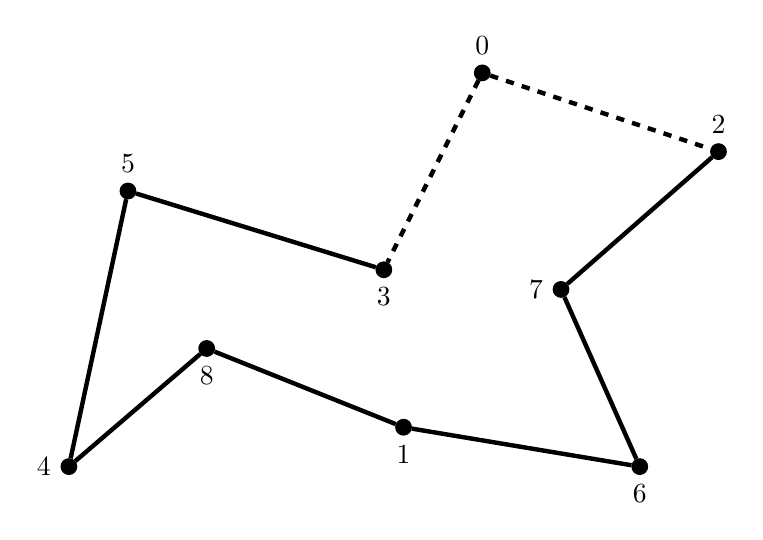
\begin{tikzpicture}
			\node[circle, draw=black, fill=black, inner sep = 2pt, label={above:0}](v0) at (2,3) {};
			\node[circle, draw=black, fill=black, inner sep = 2pt, label={below:1}](v1) at (1,-1.5) {};
			\node[circle, draw=black, fill=black, inner sep = 2pt, label={above:2}](v2) at (5,2) {};
			\node[circle, draw=black, fill=black, inner sep = 2pt, label={below:3}](v3) at (0.75,0.5) {};
			\node[circle, draw=black, fill=black, inner sep = 2pt, label={left:4}](v4) at (-3.25,-2) {};
			\node[circle, draw=black, fill=black, inner sep = 2pt, label={above:5}](v5) at (-2.5,1.5) {};
			\node[circle, draw=black, fill=black, inner sep = 2pt, label={below:6}](v6) at (4,-2) {};
			\node[circle, draw=black, fill=black, inner sep = 2pt, label={left:7}](v7) at (3,0.25) {};
			\node[circle, draw=black, fill=black, inner sep = 2pt, label={below:8}](v8) at (-1.5,-0.5) {};

			\draw[-, ultra thick] (v5) -- (v4);
			\draw[-, ultra thick] (v8) -- (v4);
			\draw[-, ultra thick] (v8) -- (v1);
			\draw[-, ultra thick] (v5) -- (v3);
			\draw[-, ultra thick] (v1) -- (v6);
			\draw[-, ultra thick] (v7) -- (v6);
			\draw[-, ultra thick] (v7) -- (v2);
			\draw[dashed, ultra thick] (v0) -- (v2);
			\draw[dashed, ultra thick] (v0) -- (v3);
		\end{tikzpicture}
	}
		\label{fig:tsp1tree3}
	}
	\caption{Exemplos de soluções para \eqref{eq:probRelaxTSP}}
\end{figure}

\subsection{Resolução do MS1TP}



% \subsection{Resolução do dual lagrangiano}
% 
% % }
% 
% \subsection{Regra de \textit{branching}}
% 
% \section{Relaxando uma restrição}
% Considere o ILP \[min \{ c^Tx \;|\; Ax \geq b\} \]
% e que 
% 
% \(A = \begin{bmatrix}
% A_1 \\
% A_2 \\
% \end{bmatrix}\) e \(b = \begin{bmatrix}
% b1 \\
% b2 \\
% 
% \end{bmatrix}\). 
% O mesmo problema pode então ser escrito como 
% \[min \{ c^Tx \;|\; A_1x \geq b_1, A_2x \geq b_2\}. \label{P_rl} \tag{P} \] Suponha que as inequações \(A_2x \geq b_2\)
% sejam consideradas restrições ``difíceis'', e que resolver uma versão de \ref{P_rl} que não possua essas restrições seja considerada uma operação muito mais fácil. Em casos como esse, convém utilizar-se a seguinte versão ``relaxada" \footnote{Diz-se ``versão relaxada'' uma variação de um problema com menos restrições que a versão original.} de \((P)\) 
% 
% \[min \{ c^Tx + \lambda (b_2 - A_2x) \;|\; A_1x \geq b_1\}.  \tag{RL}\]
% 
% Se \(A_2x < b_2\), \(x\) não é viável para \((P)\), \(\lambda (b_2 - A_2x)\) é positivo e penaliza a função objetivo, que é de minimização. A região de soluções viáveis de \((RL)\), porém, permanece muito maior do que a de \((P)\), já que o último tem mais restrições que o primeiro. Portanto, se \(x\) é viável em \((RL)\), \(x\) não necessariamente é viável em \((P)\), embora o contrário sempre seja válido.
% 
% \begin{theorem}
% A solução ótima de \((RL)\) sempre é menor ou igual à solução ótima de \((P)\) para qualquer \(\lambda \geq 0\).
% \label{teoremaLB}
% \end{theorem}
% 
% \begin{proof}
% Para qualquer \(x\), se as restrições \(A_2x \geq b_2\) não forem violadas, a FO será sempre ``recompensada'' em \((RL)\).
% \end{proof}
% 
% Portanto, para qualquer valor de \(\lambda\), resolver \((RL)\) equivale a encontrar um LB para \((P)\).
% 
% \section{Dual lagrangiano}
% Durante a resolução de \((RL)\), a solução ótima \(x^*\) depende dos valores de \(\lambda\), que são constantes no processo. Consequentemente, \(RL\) pode ser considerado uma função que depende dos valores de \(\lambda\). Mais especificamente, \(RL\) se comporta como uma função linear por partes, como demonstrado de maneira intuitiva em \cite{rl1}.
% 
% Sendo assim, o problema que consiste em encontrar os valores de \(\lambda\) que proporcionem o maior LB possível para \((P)\) pode ser entendido como
% 
% \[\{max(RL)\;|\; \lambda \geq 0 \}. \tag{D}\]
% 
% \((D)\) é conhecido como o Dual Lagrangiano. Conforme mostrado em \cite{rl1}, \((D)\) sempre possui um ótimo global, e computá-lo requer um método iterativo.
% 
% \section{Subgradientes}
% Os subgradientes podem ser interpretados como uma versão generalizada da \linebreak noção de derivada, e são úteis na análise de funções contínuas não diferenciáveis. De maneira geral, sendo \(f : \mathbb{R}^n \rightarrow \mathbb{R}\), o vetor coluna \(g \in \mathbb{R}^n\) é considerado um subgradiente no ponto \(x_0 \in \mathbb{R}^n\) se \[f(x)-f(x_0) \geq g^T(x-x_0)\] é válido para todo \(x \in \mathbb{R}^n\).
% 
% \begin{theorem}
% Se $x^*$ é uma solução ótima de \((RL_{\lambda'})\), \(Ax^* - b\) é subgradiente de \((RL_{\lambda})\) em \(\lambda'\).
% \end{theorem}
% 
% \begin{proof}
% Considere \(z\) a FO de \(RL_{\lambda}\). Então
% \begin{align*}
% z(RL_{\lambda'}) & = \text{min } c^Tx + {\lambda'}^T(b-Ax) \\
%                 & = c^Tx^* + {\lambda'}^T(b-Ax^*) \\
% z(RL_{\lambda}) & \leq c^Tx^* + \lambda^T(b-Ax^*) \\
%                 & \leq c^Tx^* + \lambda^T(b-Ax^*) + {\lambda'}^T(b-Ax^*) - {\lambda'}^T(b-Ax^*)  \\
%                 & \leq c^Tx^* + {\lambda'}^T(b-Ax^*) + (\lambda-\lambda')^T(b-Ax^*) \\
% z(RL_{\lambda}) & \leq z(RL_{\lambda'}) + (\lambda-\lambda')^T(b-Ax^*) \\
% z(RL_{\lambda}) - z(RL_{\lambda'}) & \leq  (\lambda-\lambda')^T(b-Ax^*) \\
% z(RL_{\lambda}) - z(RL_{\lambda'}) & \geq  (\lambda-\lambda')^T(Ax^* - b)
% .\end{align*}
% \end{proof}
% 
% Encontrar um vetor gradiente \(g \in \mathbb{R}^n\) de uma função \(f(x)\) em um certo ponto \( x \in \mathbb{R}^n\) garante que, avançando-se minimamente na direção de \(g\), o valor de \(f(x)\) aumenta. Analogamente, ``caminhar" na direção de \(-g\) diminui o valor de \(f(x)\).
% 
% Se houver uma maneira de computar \(g\), o Dual Lagrangiano pode então ser resolvido caminhando-se repetidamente em sua direção, até que não se possa mais aumentar o valor da função objetivo de \((D)\). 
% 
% Sabendo-se que, para quaisquer valores de \(\lambda\), \(g = Ax^* - b\) é subgradiente, \((D)\) pode ser resolvido por meio do algoritmo explicado em \cite{rl3}. Além disso, uma breve discussão acerca de bons parâmetros para o algoritmo é apresentada em \cite{nelsonmaculanmarciah.costafampa2004}.
% 
% \section{Relaxação do TSP}
% Conforme mostrado em \cite{rl2}, removendo-se as restrições de grau da formulação matemática do TSP e adicionando-se penalizações em sua FO, obtém-se uma representação implícita do problema da 1-árvore geradora mínima.
% 
% Por isso, pelo Teorema \ref{teoremaLB}, tratar uma instância do TSP como um problema da 1-árvore geradora mínima garante a obtenção de um LB.
% 
% \section{Algoritmo Kruskal}
% O algoritmo Kruskal é capaz de encontrar a árvore geradora mínima, dado um grafo. Uma implementação do algoritmo está disponível neste link: \url{https://github.com/carlosvinicius01/kit-opt/tree/master/Relaxa%C3%A7%C3%A3o-Lagrangeana/min-spanning-tree}.
% 
% Note que, para que gere uma 1-árvore geradora mínima como solução, o algoritmo deve ser modificado. Para isso, é necessário encontrar a árvore geradora mínima sem considerar o primeiro nó, e conectá-lo aos dois nós mais próximos na solução.
% 
% \section{BB com relaxação lagrangiana}
% 
% Sabendo-se que LBs podem ser obtidos resolvendo-se a versão relaxada do TSP, um algoritmo BB pode ser aplicado desde que se estabeleça um método de \textit{branching}.
% 
% Considere, então, uma 1-árvore geradora mínima obtida a partir dos custos e nós de uma instância do TSP. É necessário proibir a aparição de nós cujo grau é maior que 2 na solução --- já que as restrições que impedem que isso aconteça foram removidas. Por isso, pode-se escolher o nó conectado ao maior número de nós na solução e proibir cada uma das arestas conectadas a ele separadamente.
% 
% Um exemplo de uma 1-árvore geradora mínima para uma instância do TSP com 6 nós é mostrado na Figura \ref{fig:1arvore}. Na Figura, o nó conectado ao maior número de arestas é o nó 2. Consequentemente, gerar novas versões do problema, proibindo nelas cada uma das arestas conectadas ao nó 2 individualmente pode ser entendido como a etapa de \textit{branching}.
% 
% \begin{figure}[h]
%     \centering
%     \begin{tikzpicture}
%     
%     \node[circle, draw=black] (v2) at (2,0) {2};
%     \node[circle, draw=black] (v3) at (4,0) {3};
%     \node[circle, draw=black] (v5) at (4,-4) {5};
%     \node[circle, draw=black] (v6) at (2,-4) {6};
%     \node[circle, draw=black] (v4) at (6,-2) {4};
%     \node[circle, draw=black] (v1) at (0,-2) {1};
%     
%     \draw[-] (v1)--(v2);
%     \draw[-] (v2)--(v3);
%     \draw[-] (v2)--(v5);
%     \draw[-] (v2)--(v4);
%     \draw[-] (v6)--(v1);
%     \draw[-] (v6)--(v2);
%     
%     \end{tikzpicture} 
%     \caption{1-árvore geradora mínima.}
%     \label{fig:1arvore}
% \end{figure}
% 
% Assim, o \textit{BB} com relaxação lagrangeana pode ser feito resolvendo-se o problema da 1-árvore geradora mínima para calcular \textit{lower bounds} e utilizando-se como método de \textit{branching} a proibição das arestas conectadas ao nó de maior grau --- fazendo-se \(c_{ij} = \infty\) na matriz de instância. Além disso, durante o \textit{branching}, os nós filhos devem herdar os coeficientes de $\lambda$ associados ao melhor \textit{lower bound} do nó pai (i.e., o vetor $\lambda$ que propiciou a melhor solução durante o método do subgradiente).
% 
% \section{\textit{Benchmark}}
% 
% Os resultados apresentados abaixo foram obtidos através da utilização da meta-heurística GILS-RVND para fornecer uma boa solução $ x $ de custo $ f(x) $ para definir o limitante primal $ \overline{\mathcal{L}}$. Adotou-se  $ \overline{\mathcal{L}} = f(x) + 1 $ , visando provar a eficácia do algoritmo em casos onde $ f(x) = f(x^*)$.
% 
% \begin{table}[!ht]
%  \centering
%  \caption{Resultados}
%  \footnotesize
%  \begin{tabular}{ccc}
%  \toprule
% \multirow{2.5}{*}{\textbf{Instância}} & \multicolumn{2}{c}{\textbf{Resultados}} \\
% \cmidrule{2-3} & \textbf{Tempo} & \textbf{Custo} \\
% \midrule
%     \texttt{att48}      & 1.80368         & 10628          \\
%     \texttt{bayg29}     & 0.007836        & 1610           \\
%     \texttt{bays29}     & 0.238564        & 2020           \\
%     \texttt{berlin52}   & 2e-06           & 7542           \\
%     \texttt{brazil58}   & 9.7251          & 25395          \\
%     \texttt{burma14}    & 3e-06           & 3323           \\
%     \texttt{dantzig42}  & 0.212829        & 699            \\
%     \texttt{fri26}      & 0.0025          & 937            \\
%     \texttt{gr17}       & 2e-06           & 2085           \\
%     \texttt{gr21}       & 1e-06           & 2707           \\
%     \texttt{gr24}       & 0.071051        & 1272           \\
%     \texttt{gr48}       & 186.834         & 5046           \\
%     \texttt{hk48}       & 0.198611        & 11461          \\
%     \texttt{lin105}     & 14.4901         & 14379          \\
%     \texttt{rat99}      & 53.8981         & 1211           \\
%     \texttt{st70}       & 21.3005         & 675            \\
%     \texttt{swiss42}    & 0.949663        & 1273           \\
%     \texttt{ulysses16}  & 2e-06           & 6859           \\
%     \texttt{ulysses22}  & 0.00699         & 7013           \\
% \bottomrule
%  \end{tabular}
%  \label{tab:rLagResults}
%  \end{table}
% 
